\documentclass[a4paper,11pt,dvipdfmx]{ujarticle}
% パッケージ
\usepackage{graphicx}
\usepackage{url}
% レイアウト指定を記述したファイルの読み込み
\input{layout}

\title{日本におけるデジタル化の状況}
\author{G685122026 米山 潤}

\begin{document}

\maketitle %ここにタイトルが入る

\section{デジタル競争力ランキング}

国際経営開発研究所(IMD)の調査\cite{imd}によると，
日本のデジタル競争力のランキングは図\ref{fig:ランキング}に示すように，
調査対象の64カ国中，総合で28位，技術分野で30位となっている．

\begin{figure}[htbp]
    \centering
    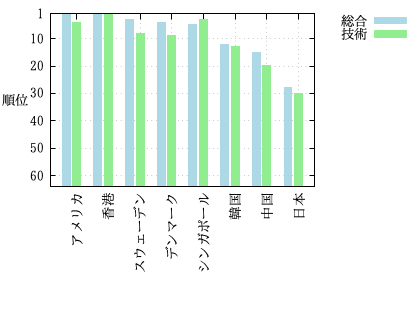
\includegraphics[width=0.7\linewidth]{fig41.png}
    \caption{デジタル競争力ランキング(64カ国中)}\label{fig:ランキング}
\end{figure}

\section{ブロードバンドの整備状況}

OECDによるブロードバンド回線の普及に関する調査\cite{oecd}によると，
表\ref{tbl:加入者数}に示すように，
日本における100人あたりの光ファイバー回線の加入者数は29.0で，
韓国，スウェーデン，ノルウェーに続いて第4位になっている．

\begin{table}[htbp]
    \centering
    \caption{光ファイバー回線の加入者数(100人あたり)}
    \label{tbl:加入者数}

    \begin{tabular}{|c|l|r|}\hline
        順位 & 国名 & 加入者数 \\
        \hline
        1位 & 韓国 & 38.2 \\
        \hline
        2位 & スウェーデン & 31.9 \\
        \hline
        3位 & ノルウェー & 29.5 \\
        \hline
        4位 & 日本 & 29.0 \\
        \hline
        5位 & アイスランド & 28.8 \\
        \hline
        6位 & スペイン & 27.3 \\
        \hline
        7位 & ポルトガル & 25.1 \\
        \hline
        8位 & ニュージーランド & 23.6 \\
        \hline
        9位 & リトアニア & 22.3 \\
        \hline
        10位 & フランス & 21.2 \\
        \hline
    \end{tabular}
\end{table}

\section{考察}

\begin{itemize}
    \item 日本は光ファイバー回線の加入者数が世界第4位であり，通信インフラの整備は世界的に見ても高い水準にある．
    \item 一方で，デジタル競争力は総合28位，技術分野でも30位にとどまっており，整備されたインフラを十分に活用できていないと考えられる．
    \item インフラの整備状況と競争力の順位に差があることから，今後はデジタル人材の育成や，行政・企業のデジタル活用の推進が課題になると考える．
\end{itemize}

\bibliographystyle{junsrt}
\bibliography{exercise.bib}

\end{document}
